% !TeX program = xelatex
\documentclass[UTF8,a4paper,zihao=-4,fontset=none]{ctexart}
\usepackage[left=35mm,right=30mm,top=25mm,bottom=25mm,footskip=12mm]{geometry}
\usepackage{fontspec}
\setmainfont{Times New Roman}
\setsansfont{Arial}
\setCJKmainfont{SimSun}[BoldFont=SimHei,ItalicFont=KaiTi]
\setCJKsansfont{SimHei}
\setCJKmonofont{SimSun}
\setCJKfamilyfont{kai}{KaiTi}
\providecommand{\songti}{\rmfamily}
\providecommand{\heiti}{\sffamily}
\usepackage{amsmath}
\usepackage{unicode-math}
\setmathfont{TeX Gyre Termes Math}
\usepackage{graphicx,booktabs,array,tabularx,longtable,multirow}
\usepackage{caption,subcaption,float,placeins}
\usepackage{tikz,eso-pic}
\usepackage[hidelinks,unicode,bookmarksnumbered]{hyperref}
\usepackage{xurl}
\usepackage{enumitem}
\usepackage{fancyhdr}
\usepackage{microtype}
\graphicspath{{../figures/generated/}{../references/images/}{assets/}}
\hypersetup{pdftitle={五杆绘图机器人的串并联运动学与动力学建模分析},pdfauthor={张子安琪},pdfsubject={机器人动力学基础结课报告}}
\ctexset{section={format=\heiti\zihao{4},name={,、},number=\chinese{section},aftername=\hspace{0pt},beforeskip=16pt,afterskip=8pt},subsection={format=\heiti\zihao{-4},beforeskip=12pt,afterskip=6pt},subsubsection={format=\heiti\zihao{-4},beforeskip=10pt,afterskip=4pt}}
\renewcommand{\thesubsection}{\arabic{section}.\arabic{subsection}}
\renewcommand{\thesubsubsection}{\arabic{section}.\arabic{subsection}.\arabic{subsubsection}}
\renewcommand{\theequation}{\arabic{section}-\arabic{equation}}
\makeatletter\@addtoreset{equation}{section}\makeatother
\captionsetup{font=small,labelfont=normalfont,labelsep=quad,skip=5pt}
\captionsetup[figure]{name=图}
\captionsetup[table]{name=表,position=top}
\setlength{\parindent}{2em}
\setlength{\parskip}{0pt}
\linespread{1}
\setlength{\abovedisplayskip}{7pt plus 2pt minus 2pt}
\setlength{\belowdisplayskip}{7pt plus 2pt minus 2pt}
\setlength{\textfloatsep}{12pt plus 3pt minus 2pt}
\setlength{\intextsep}{12pt plus 3pt minus 2pt}
\renewcommand{\topfraction}{0.9}
\renewcommand{\bottomfraction}{0.8}
\renewcommand{\textfraction}{0.08}
\renewcommand{\floatpagefraction}{0.76}
\setcounter{topnumber}{3}
\setcounter{bottomnumber}{2}
\setcounter{totalnumber}{4}
\emergencystretch=2em
\setlist{nosep,leftmargin=2em}
\pagestyle{fancy}\fancyhf{}\fancyfoot[C]{\small\thepage}
\renewcommand{\headrulewidth}{0pt}
\newcommand{\vect}[1]{\symbfit{#1}}
\newcommand{\dd}{\mathrm d}
\newcommand{\R}{\mathbb R}
\newcommand{\T}{\mathsf T}
\newcommand{\e}{\mathrm e}
\newcommand{\units}[1]{\,\mathrm{#1}}
\newcommand{\figfull}[3]{\begin{figure}[htbp]\centering\includegraphics[width=\linewidth]{#1}\caption{#2}\label{#3}\end{figure}}
\begin{document}
\fontsize{12pt}{18pt}\selectfont
\thispagestyle{empty}
\AddToShipoutPictureBG*{\AtPageLowerLeft{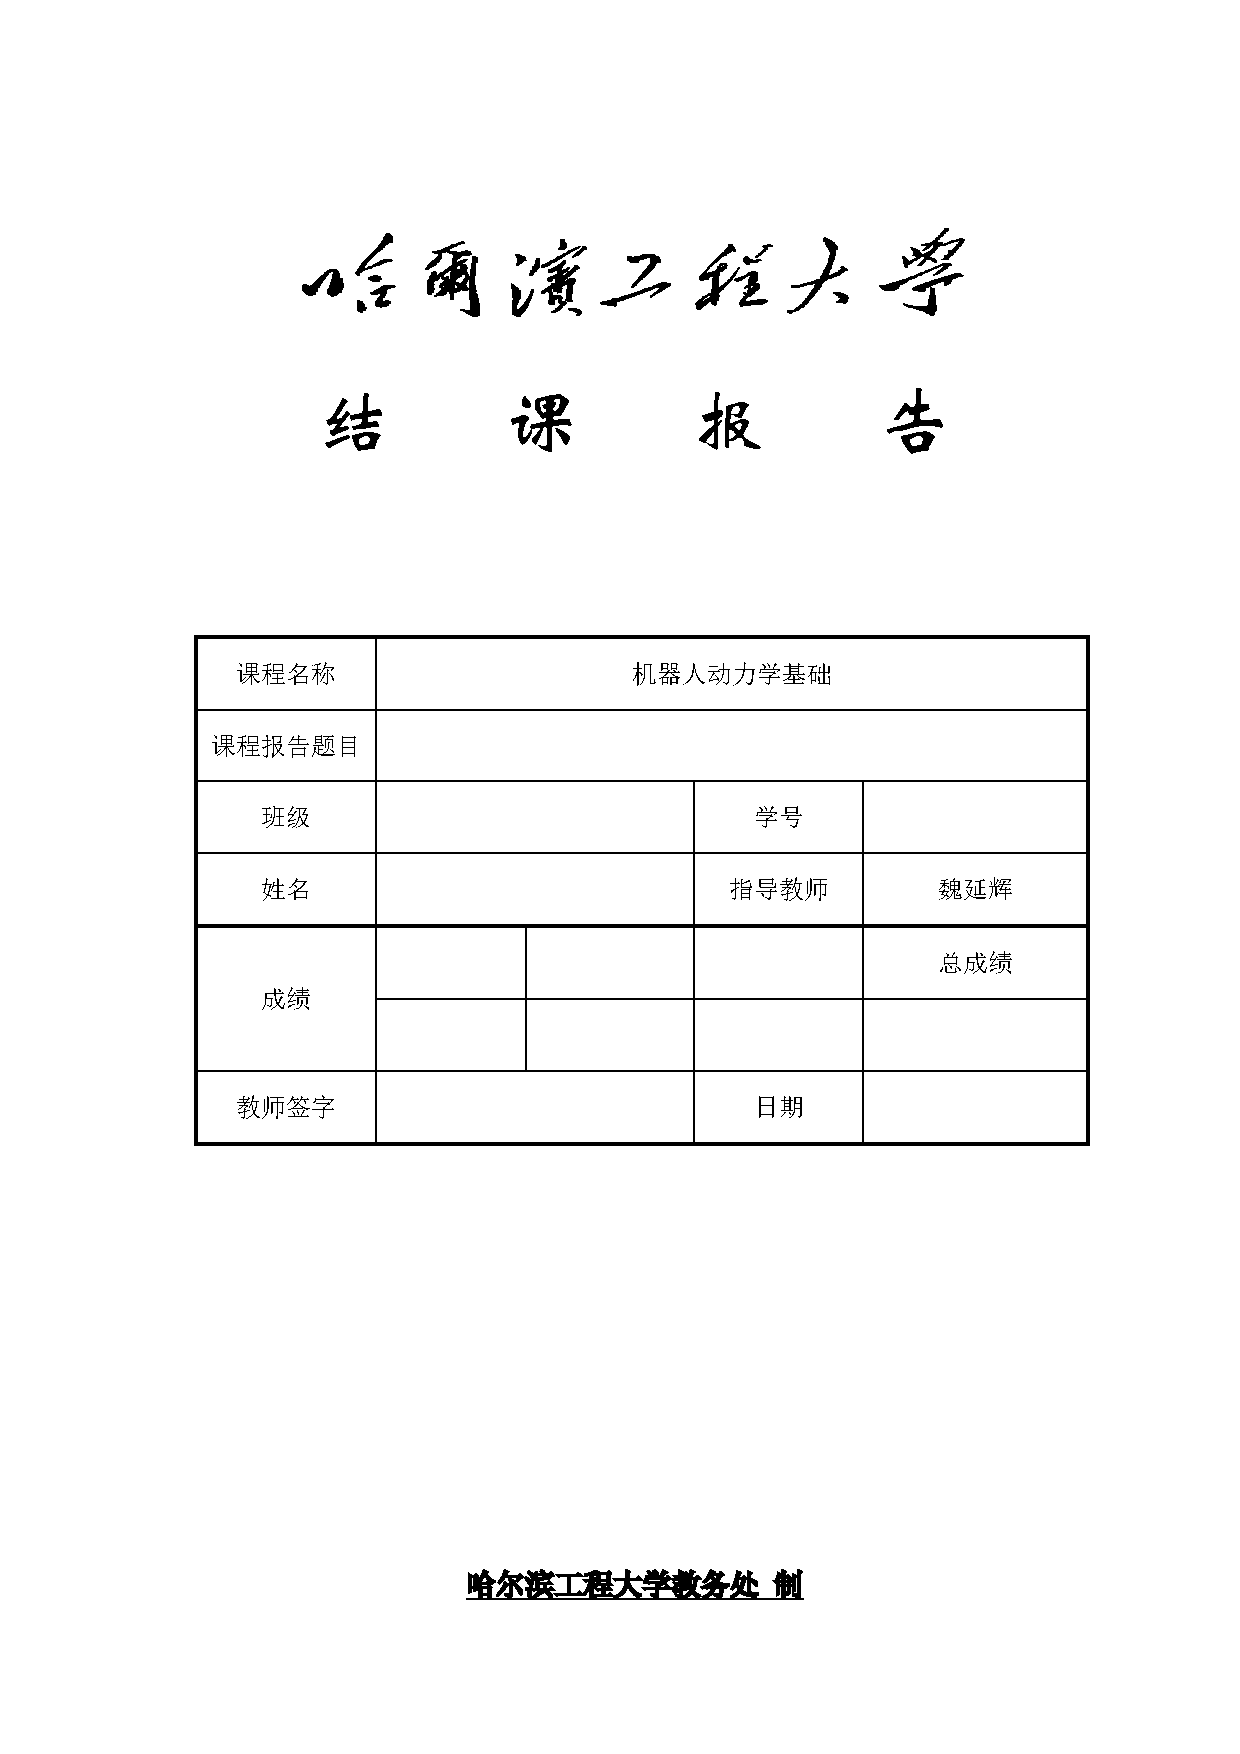
\includegraphics[width=\paperwidth,height=\paperheight]{assets/cover_background.pdf}}}
\begin{tikzpicture}[remember picture,overlay]
\node[align=center,font=\songti\fontsize{11pt}{14pt}\selectfont] at ([xshift=351.3bp,yshift=-358.0bp]current page.north west) {五杆绘图机器人的串并联运动学\\与动力学建模分析};
\node[font=\fontsize{12pt}{18pt}\selectfont] at ([xshift=258.2bp,yshift=-392.4bp]current page.north west) {20240414};
\node[font=\fontsize{12pt}{18pt}\selectfont] at ([xshift=469.8bp,yshift=-392.4bp]current page.north west) {2024079102};
\node[font=\songti\fontsize{12pt}{18pt}\selectfont] at ([xshift=258.2bp,yshift=-427.0bp]current page.north west) {张子安琪};
\node[font=\fontsize{12pt}{18pt}\selectfont] at ([xshift=469.8bp,yshift=-531.6bp]current page.north west) {2026.10.25};
\end{tikzpicture}
\null\newpage

\setcounter{page}{1}
\begin{center}
{\heiti\fontsize{22pt}{29pt}\selectfont 五杆绘图机器人的串并联运动学\\与动力学建模分析\par}
\vspace{8pt}
{\CJKfamily{kai} 张子安琪\par}
\end{center}
\vspace{5pt}
\noindent{\heiti\zihao{4} 摘\quad 要：}\!以Quanser五杆绘图机器人的机构拓扑与笔式绘迹应用为参照，建立竖直板面椭圆轮廓描绘的课程设计模型，分析串联支链与并联整机的运动及负载关系。首先采用DH方法推导2R串联支链的正逆运动学与位置雅可比，基于动能和势能建立拉格朗日动力学，并用独立牛顿—欧拉递推进行核验；随后推导五杆机构的闭环正逆解、速度约束和奇异性条件，通过虚功将支链动力学投影为两个主动关节的整机动力学。Python计算表明，500组随机状态下两种串联动力学实现的最大扭矩差为$1.78\times10^{-15}\units{N\,m}$，高精度正动力学回放的末端最大偏差为$3.42\times10^{-8}\units m$。常规轨迹与近奇异轨迹的并联雅可比最大条件数分别约为5.56和273；在相同$1\units N$竖直等效力下，两个代表位形的单电机力矩幅值分别为0.896和$41.54\units{N\,m}$。结果说明，几何可达并不保证良好的传力性能，轮廓位置选择必须结合闭环奇异性评价。本文结果限于设定参数下的理想刚体仿真，可为绘图机构的轨迹布置与驱动负载分析提供可复现的课程算例。

\vspace{6pt}
\noindent{\heiti\zihao{4} 关键词：}\!五杆绘图机器人；串联与并联；雅可比矩阵；拉格朗日方程；牛顿—欧拉方程；奇异性
\vspace{5pt}

\section{引言}

机器人完成一条指定轮廓，既需要求出末端位置与关节角的对应关系，也需要计算驱动器应提供的力矩。正运动学回答“给定关节角，末端在哪里”，逆运动学回答“到达目标点需要怎样的关节角”，雅可比矩阵则把这两类位置关系延伸到速度与力的映射。动力学进一步考虑质量、转动惯量和重力，使轨迹规划能够与驱动负载联系起来。对于并联机器人，还必须满足多条支链在同一末端处的闭环约束。因此，仅展示一条能够画出的曲线，尚不足以说明机器人能够平稳、可靠地执行该任务。

本文选择具有实际绘图和教学应用背景的平面五杆机器人，研究其在竖直工件板面上描绘椭圆轮廓的设计问题。实物平台与设计场景的对应关系在第2.1节说明。五杆机构由两条2R串联支链连接同一末端构成，既保留双连杆运动的直观几何关系，又包含闭链机构特有的工作模式、装配模式和并联奇异性，适合在同一案例中贯通课程内容。MIT机器人课程讲义直接以五杆机构说明串联支链组成并联机构的方式；Modern Robotics则提供运动学、静力学和受约束动力学的统一框架\cite{asada2005,lynch2017}。

针对五杆机构，已有研究系统讨论了对称5R机构的运动学、奇异性与工作空间\cite{liu2006}。这些理论提示了一个与实际描绘任务直接相关的问题：目标点虽然位于几何可达域内，机构仍可能接近闭环奇异位形，导致速度、误差和驱动力矩的映射显著恶化。本文不提出新的机构理论，而是围绕这一问题完成可核查的推导和计算：先将左侧支链作为独立2R开链，建立DH运动学、雅可比及拉格朗日动力学；再以独立牛顿—欧拉递推进行交叉核验；随后恢复五杆闭环，推导并联正逆解与两类奇异性，并通过虚功把支链动力学组装为整机模型；最后比较常规描绘轨迹与近奇异轨迹，分析工作空间选择对驱动负载的影响。

\section{系统建模与理论推导}

\subsection{实际机器人背景、任务场景与参数}
\label{sec:system}

实际参照平台为Quanser公司的2 DOF Planar Robot绘图实验机器人，如图\ref{fig:real_robot}所示。制造商介绍与用户手册表明，该设备采用五杆并联机构，两台带减速器的电机驱动基座关节，公共末端安装笔，并由电磁机构完成落笔，以纸上轨迹展示机器人运动效果\cite{barnard2009,quanser2013}。因此，轮廓描绘不仅是抽象的点轨迹，也对应真实设备中的笔尖定位任务。

\begin{figure}[htbp]
\centering
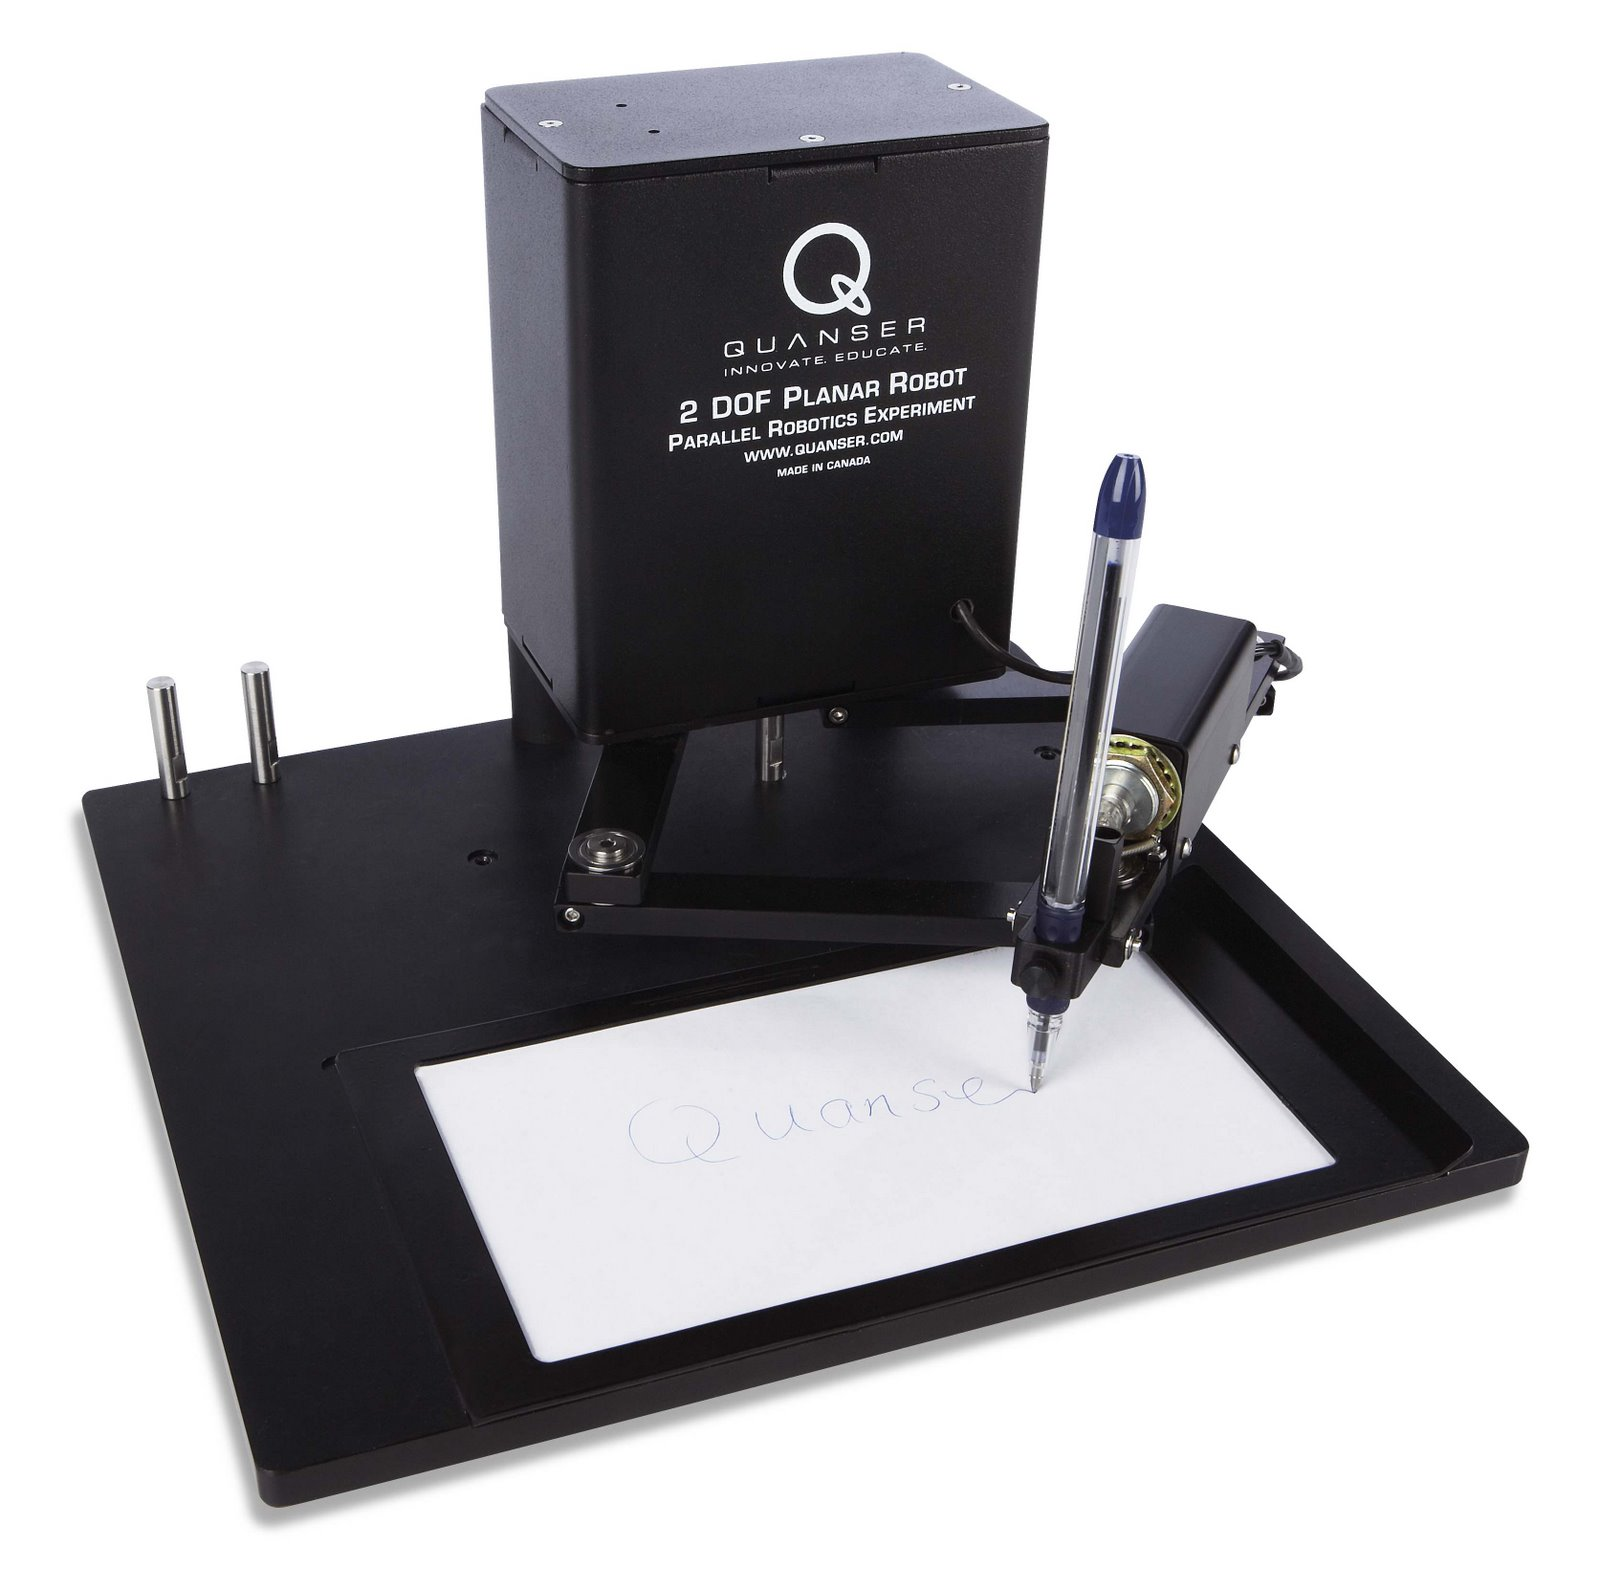
\includegraphics[width=0.66\linewidth]{Quanser_2009_2DOF_Planar_Robot_official_blog.jpg}
\caption{Quanser 2 DOF Planar Robot实物及笔式绘迹配置。来源：制造商官方工程博客，Barnard，2009\cite{barnard2009}；\textcopyright\ Quanser，原图未修改，作为实际机构与应用场景的引用图片。}
\label{fig:real_robot}
\end{figure}

本文保留该平台的五杆拓扑与笔式绘迹需求，进一步设定一个竖直工件板上的椭圆轮廓标记场景：工具在宽$80\units{mm}$、高$50\units{mm}$的轮廓上运动，并在$4\units s$内从静止出发、闭合后回到静止。与桌面绘图相比，竖直安装使杆件和工具的重力直接参与板面内负载，适合分析拉格朗日和牛顿—欧拉方程中的重力项。表\ref{tab:parameters}所列尺寸、质量及安装方向均为本报告的课程设计输入，未将其标作Quanser原机规格，也不将数值仿真表述为原机实测或参数复现。

在工程实施中，完整描绘流程还包括定位板面、抬笔到起点、落笔、沿轮廓运动与抬笔退出。本文研究其中落笔后的二维轮廓段；法向落笔行程作为独立动作，不引入二维模型的自由度。安装方向的影响将在第3节用同一机构从水平到竖直的倾角扫描进行定量说明。


\begin{figure}[htbp]
\centering
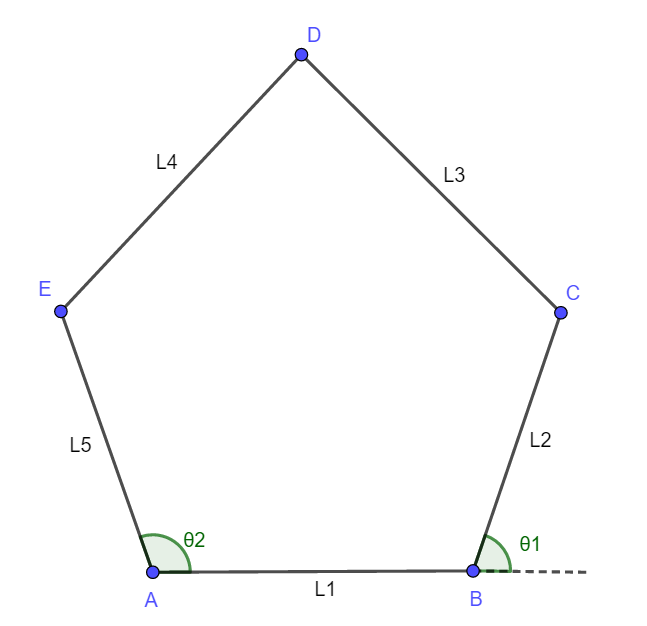
\includegraphics[width=0.57\linewidth]{Five_bar_mechanism_I_Elgamal_2020.png}
\caption{五杆闭链机构的公开示意图。原作者I.Elgamal，2020，原图未修改\cite{elgamal2020}；采用\href{https://creativecommons.org/licenses/by-sa/4.0/}{CC BY-SA 4.0}许可。原图字母与本文建模符号分别定义。}
\label{fig:external}
\end{figure}

本文模型如图\ref{fig:model}所示，固定基座为$A=(-d/2,0)^\T$和$B=(d/2,0)^\T$，肘关节为$C$、$D$，末端公共转动副为$P$。两侧近杆长度均为$l_1$，远杆长度均为$l_2$。世界坐标$x$向右、$y$向上，所有角度逆时针为正。机架$AB$与四根运动杆共五个构件，五个转动副约束平面刚体运动，自由度为
\begin{equation}
F=3(n-1)-2j=3(5-1)-2\times5=2.
\end{equation}
该计数适用于一般非退化位形；奇异位形还须检查约束矩阵的秩。驱动器位于$A$、$B$，两个主动角记为$\vect\theta=(\theta_L,\theta_R)^\T$。左、右支链各用相对关节坐标$\vect q_i=(q_{1i},q_{2i})^\T$表示，其中$q_{1L}=\theta_L$、$q_{1R}=\theta_R$，远杆绝对角为$q_{1i}+q_{2i}$。末端只控制平面位置，不能另外独立指定工具在平面内的姿态。

\figfull{fig01_mechanism.pdf}{本文五杆机器人设计模型。两主动关节位于固定基座，$q_{2L}$为左支链相对角；长度与质量采用表\ref{tab:parameters}中的课程设计值。}{fig:model}

\begin{table}[htbp]
\centering\caption{课程设计模型参数与物理含义}\label{tab:parameters}
\small\begin{tabularx}{\linewidth}{@{}lclX@{}}
\toprule 参数 & 符号 & 数值 & 说明\\\midrule
基座间距 & $d$ & $0.36\units m$ & 两驱动转轴中心距\\
近杆长度 & $l_1$ & $0.32\units m$ & $AC$、$BD$\\
远杆长度 & $l_2$ & $0.28\units m$ & $CP$、$DP$\\
近杆质量 & $m_1$ & $0.80\units{kg}$ & 每根近杆各一份\\
远杆质量 & $m_2$ & $0.60\units{kg}$ & 每根远杆各一份\\
工具等效质量 & $m_p$ & $0.25\units{kg}$ & 末端笔及夹持组件的点质量\\
质心位置 & $r_1,r_2$ & $0.16,0.14\units m$ & 均匀细杆中点\\
质心转动惯量 & $I_1,I_2$ & $0.006827,0.003920\units{kg\,m^2}$ & $I_i=m_i l_i^2/12$\\
重力加速度 & $g_0$ & $9.81\units{m/s^2}$ & 竖直板面内方向为$-y$\\
轮廓执行时间 & $T_f$ & $4.00\units s$ & 单次闭合椭圆描绘\\\bottomrule
\end{tabularx}
\end{table}

为使推导与数值检验保持一致，假设杆件刚性、关节无摩擦且无间隙，忽略电机转子惯量、减速器弹性和关节限位。工具简化为无自转惯量的点质量；纸面法向接触由独立压笔机构承担，本文只研究板面内的位置与负载，不建立接触摩擦模型。四根运动杆总质量为$2(m_1+m_2)=2.8\units{kg}$，整机运动部分加工具为$3.05\units{kg}$。

后续有两个不同的力学问题。串联部分将左支链解除闭环，作为带末端质量$m_p$的独立2R机器人，两关节均视为可驱动。并联部分恢复右支链，只有两个基座关节主动驱动，末端质量在整机中只计一次。因此，开链的$(\tau_1,\tau_2)$与整机的$(\tau_L,\tau_R)$具有不同物理含义，不能直接相互替代。

\subsection{2R串联支链的正逆运动学}
\label{sec:serial_kinematics}

\subsubsection{坐标建立与DH变换}

取左基座$A$为局部原点，两个转轴均垂直于运动平面。采用标准DH记号\cite{denavit1955}，即$\operatorname{Rot}_z(\theta_i)\operatorname{Trans}_z(d_i)\operatorname{Trans}_x(a_i)\operatorname{Rot}_x(\alpha_i)$，参数见表\ref{tab:dh}。
\begin{table}[htbp]
\centering\caption{左侧2R支链的标准DH参数}\label{tab:dh}
\begin{tabular}{ccccc}\toprule 连杆$i$ & $a_i$ & $\alpha_i$ & $d_i$ & $\theta_i$\\\midrule
1 & $l_1$ & 0 & 0 & $q_1$\\
2 & $l_2$ & 0 & 0 & $q_2$\\\bottomrule\end{tabular}
\end{table}
令$c_i=\cos q_i$、$s_i=\sin q_i$，单杆齐次变换为
\begin{equation}
{}^{i-1}\vect T_i=
\begin{bmatrix}
c_i&-s_i&0&l_i c_i\\s_i&c_i&0&l_i s_i\\0&0&1&0\\0&0&0&1
\end{bmatrix}.
\end{equation}
相乘$\vect T_{02}=\vect T_{01}\vect T_{12}$，并令$c_{12}=\cos(q_1+q_2)$、$s_{12}=\sin(q_1+q_2)$，得到
\begin{equation}
\vect T_{02}=\begin{bmatrix}
c_{12}&-s_{12}&0&l_1 c_1+l_2 c_{12}\\
s_{12}&c_{12}&0&l_1 s_1+l_2 s_{12}\\
0&0&1&0\\0&0&0&1
\end{bmatrix}.
\end{equation}
故世界坐标中的末端位置为
\begin{equation}
\vect p=\vect A+
\begin{bmatrix}l_1\cos q_1+l_2\cos(q_1+q_2)\\l_1\sin q_1+l_2\sin(q_1+q_2)\end{bmatrix}.
\label{eq:fk}
\end{equation}
基座平移不会改变位置雅可比，但会影响逆解中使用的目标坐标，计算时必须先减去$\vect A$。

\subsubsection{解析逆解与多解处理}

令$(X,Y)^\T=\vect p-\vect A$，由余弦定理可得
\begin{align}
c_2&=\frac{X^2+Y^2-l_1^2-l_2^2}{2l_1l_2},\\
q_2&=\operatorname{atan2}\!\left(\sigma\sqrt{1-c_2^2},c_2\right),\quad \sigma\in\{-1,1\},\\
q_1&=\operatorname{atan2}(Y,X)-\operatorname{atan2}(l_2\sin q_2,l_1+l_2\cos q_2).
\label{eq:ik}
\end{align}
存在实数解的条件为
\begin{equation}
|l_1-l_2|\leq\sqrt{X^2+Y^2}\leq l_1+l_2.
\label{eq:reach}
\end{equation}
除边界退化情况外，两种$\sigma$对应两种肘部构型。本文左支链固定$q_{2L}<0$，右支链固定$q_{2R}>0$，构成肘部向外的工作模式。逐点计算时还需保持角度连续，不能任意切换逆解分支。代码只对浮点舍入造成的微小$c_2$越界进行裁剪；真正不满足式\eqref{eq:reach}的点直接标记为不可达。

\subsection{雅可比矩阵、静力映射与可操作性}
\label{sec:jacobian}

对式\eqref{eq:fk}求时间导数，得到末端速度与关节速度的关系
\begin{equation}
\dot{\vect p}=\vect J(\vect q)\dot{\vect q},\quad
\vect J=\begin{bmatrix}
-l_1s_1-l_2s_{12}&-l_2s_{12}\\
l_1c_1+l_2c_{12}&l_2c_{12}
\end{bmatrix}.
\label{eq:jac}
\end{equation}
其中$\vect J$是$2\times2$位置雅可比，单位为$\mathrm{m/rad}$。其行列式
\begin{equation}
\det\vect J=l_1l_2\sin q_2
\end{equation}
与$q_1$无关。当$q_2=0$或$\pi$时，两杆共线，机器人失去一个瞬时位置运动方向。非奇异区域可以求解
\begin{align}
\dot{\vect q}&=\vect J^{-1}\dot{\vect p},\\
\ddot{\vect q}&=\vect J^{-1}\left(\ddot{\vect p}-\dot{\vect J}\dot{\vect q}\right).
\label{eq:qdd}
\end{align}
加速度映射中的$\dot{\vect J}\dot{\vect q}$反映几何映射随姿态变化产生的速度二次项，遗漏这一项会直接改变逆动力学扭矩。程序通过线性方程求解器实现以上关系，避免显式计算矩阵逆。

虚功相等给出速度映射对应的静力关系。若$\vect f$为末端需由关节承担的等效力，则
\begin{equation}
\vect\tau^\T\delta\vect q=\vect f^\T\delta\vect p,
\qquad \vect\tau=\vect J^\T\vect f.
\label{eq:virtual_serial}
\end{equation}
这里的$\vect f$是所需支撑或驱动的等效力；若使用“环境施加给机器人”的外力，则需按动力学平衡约定处理其符号。

依据Yoshikawa的可操作度定义\cite{yoshikawa1985}，本例方阵位置雅可比有
\begin{equation}
w=\sqrt{\det(\vect J\vect J^\T)}=|\det\vect J|=l_1l_2|\sin q_2|.
\end{equation}
另以二范数条件数$\kappa_2(\vect J)=\sigma_{\max}/\sigma_{\min}$描述方向各向异性。$w$衡量速度椭圆的面积尺度，$\kappa_2$衡量长短轴之比，二者不能互相替代。本文两个输出都是长度，比较位置雅可比的条件数不存在位置与姿态混合量纲的问题；若纳入姿态自由度，需另行规定归一化尺度。

\figfull{fig04_serial_singularity.pdf}{2R支链的可操作度与条件数随相对关节角变化。两杆共线时位置映射退化；可操作度与条件数分别反映映射尺度与方向性。}{fig:serial_singularity}

\subsection{基于拉格朗日方程的串联动力学}
\label{sec:lagrange}

\subsubsection{质心运动与能量表达式}

取广义坐标$\vect q=(q_1,q_2)^\T$。两个质心相对左基座的位置为
\begin{align}
\vect p_{c1}&=r_1\begin{bmatrix}c_1\\s_1\end{bmatrix},\\
\vect p_{c2}&=l_1\begin{bmatrix}c_1\\s_1\end{bmatrix}+r_2\begin{bmatrix}c_{12}\\s_{12}\end{bmatrix}.
\end{align}
两杆绝对角速度分别为$\omega_1=\dot q_1$、$\omega_2=\dot q_1+\dot q_2$，从而
\begin{align}
v_{c1}^2&=r_1^2\dot q_1^2,\\
v_{c2}^2&=l_1^2\dot q_1^2+r_2^2(\dot q_1+\dot q_2)^2
+2l_1r_2\cos q_2\dot q_1(\dot q_1+\dot q_2),\\
v_P^2&=l_1^2\dot q_1^2+l_2^2(\dot q_1+\dot q_2)^2
+2l_1l_2\cos q_2\dot q_1(\dot q_1+\dot q_2).
\end{align}
总动能包含杆件质心平动、自转和工具平动：
\begin{equation}
K=\frac12m_1v_{c1}^2+\frac12I_1\dot q_1^2
+\frac12m_2v_{c2}^2+\frac12I_2(\dot q_1+\dot q_2)^2+\frac12m_pv_P^2.
\end{equation}
以基座水平线为势能零位，势能为
\begin{equation}
U=g_0\left\{[m_1r_1+(m_2+m_p)l_1]\sin q_1
+(m_2r_2+m_pl_2)\sin(q_1+q_2)\right\}.
\label{eq:potential}
\end{equation}
由于角度从水平$+x$轴起算，势能使用正弦，求导后的重力项使用余弦。若照搬以竖直向下为零位的双摆公式，会产生不一致的重力方向。

\subsubsection{惯性、速度耦合与重力项}

令$L=K-U$，第二类拉格朗日方程\cite{lynch2017,asada2005}为
\begin{equation}
\frac{\dd}{\dd t}\left(\frac{\partial L}{\partial\dot q_i}\right)
-\frac{\partial L}{\partial q_i}=\tau_i,\qquad i=1,2.
\end{equation}
为展示整理过程，定义常数
\begin{align}
a_m&=I_1+I_2+m_1r_1^2+m_2(l_1^2+r_2^2)+m_p(l_1^2+l_2^2),\\
b_m&=m_2l_1r_2+m_pl_1l_2,\\
d_m&=I_2+m_2r_2^2+m_pl_2^2.
\end{align}
于是动能写成
\begin{equation}
K=\frac12(a_m+2b_m\cos q_2)\dot q_1^2
+(d_m+b_m\cos q_2)\dot q_1\dot q_2+\frac12d_m\dot q_2^2.
\end{equation}
例如第一坐标的时间导数为
\begin{align}
\frac{\dd}{\dd t}\frac{\partial K}{\partial\dot q_1}
={}&(a_m+2b_mc_2)\ddot q_1+(d_m+b_mc_2)\ddot q_2\notag\\
&-2b_ms_2\dot q_1\dot q_2-b_ms_2\dot q_2^2,
\end{align}
而$\partial K/\partial q_1=0$。对第二坐标整理后，得到标准机械臂方程
\begin{equation}
\boxed{\vect M(\vect q)\ddot{\vect q}+\vect C(\vect q,\dot{\vect q})\dot{\vect q}+\vect g(\vect q)=\vect\tau.}
\label{eq:serial_dyn}
\end{equation}
各项分别为
\begin{align}
\vect M&=\begin{bmatrix}a_m+2b_mc_2&d_m+b_mc_2\\d_m+b_mc_2&d_m\end{bmatrix},\label{eq:mass}\\
\vect C&=b_ms_2\begin{bmatrix}-\dot q_2&-(\dot q_1+\dot q_2)\\\dot q_1&0\end{bmatrix},\label{eq:coriolis}\\
\vect g&=g_0\begin{bmatrix}
[m_1r_1+(m_2+m_p)l_1]c_1+(m_2r_2+m_pl_2)c_{12}\\
(m_2r_2+m_pl_2)c_{12}
\end{bmatrix}.
\label{eq:gravity}
\end{align}
表\ref{tab:parameters}给出$a_m=0.1496267$、$b_m=0.04928$、$d_m=0.03528\units{kg\,m^2}$。惯性矩阵对称，非对角项说明一个关节的加速度也会影响另一个关节的驱动力矩。$\vect C\dot{\vect q}$含科里奥利与离心耦合，不能在双关节运动时只按两根独立单摆计算。

$\vect C$的矩阵表示并不唯一。本文采用Christoffel形式，满足$\dot{\vect M}-2\vect C$反对称，因此
\begin{equation}
\frac{\dd}{\dd t}(K+U)=\dot{\vect q}^\T\vect\tau.
\label{eq:power_serial}
\end{equation}
这一性质同时提供了数值能量检验依据。因为模型包含重力及外部驱动，运动过程中机械能通常不恒定；应比较机械能变化与累计驱动功，而不是简单要求能量曲线为水平线。

\subsubsection{逆动力学与正动力学}

逆动力学给定$\vect q(t),\dot{\vect q}(t),\ddot{\vect q}(t)$，直接由式\eqref{eq:serial_dyn}求$\vect\tau(t)$。正动力学则给定状态和驱动力矩，求解
\begin{equation}
\ddot{\vect q}=\vect M^{-1}\left(\vect\tau-\vect C\dot{\vect q}-\vect g\right).
\end{equation}
令$\vect z=(\vect q^\T,\dot{\vect q}^\T)^\T$，可转化为一阶常微分方程进行数值积分。本文将解析规划轨迹的逆动力学力矩作为连续时间输入，再由正动力学积分重建轨迹，以检验公式和实现的一致性。此过程没有位置反馈，属于理想模型的开环回放，不构成实体系统的跟踪控制试验。

\subsection{基于牛顿—欧拉方程的独立动力学推导}
\label{sec:ne}

拉格朗日方法从能量出发，牛顿—欧拉方法从逐杆受力与转动平衡出发。经典递推计算按“基座至末端求运动量、末端至基座求力和力矩”的顺序组织\cite{luh1980,lynch2017}。本例使用二维向量独立实现后者，避免仅把同一组$\vect M,\vect C,\vect g$换一个函数名称而误称为方法互证。

定义$\vect u(\psi)=(\cos\psi,\sin\psi)^\T$，$\vect t(\psi)=(-\sin\psi,\cos\psi)^\T$，平面叉积为$\vect a\times\vect b=a_xb_y-a_yb_x$。相应转速、角加速度为
\begin{equation}
\omega_1=\dot q_1,\quad\omega_2=\dot q_1+\dot q_2,\quad
\alpha_1=\ddot q_1,\quad\alpha_2=\ddot q_1+\ddot q_2.
\end{equation}
先计算质心、肘点和末端加速度：
\begin{align}
\vect a_{c1}&=r_1[\alpha_1\vect t(q_1)-\omega_1^2\vect u(q_1)],\\
\vect a_C&=l_1[\alpha_1\vect t(q_1)-\omega_1^2\vect u(q_1)],\\
\vect a_{c2}&=\vect a_C+r_2[\alpha_2\vect t(q_1+q_2)-\omega_2^2\vect u(q_1+q_2)],\\
\vect a_P&=\vect a_C+l_2[\alpha_2\vect t(q_1+q_2)-\omega_2^2\vect u(q_1+q_2)].
\label{eq:ne_acc}
\end{align}
其中第一项沿切向，第二项为向心加速度。取真实重力向量$\vect g_v=(0,-g_0)^\T$，定义扣除重力后的所需惯性合力
\begin{equation}
\vect f_1=m_1(\vect a_{c1}-\vect g_v),\quad
\vect f_2=m_2(\vect a_{c2}-\vect g_v),\quad
\vect f_p=m_p(\vect a_P-\vect g_v).
\end{equation}
从末端向基座作力矩平衡，先得到第二关节力矩
\begin{equation}
\tau_2=I_2\alpha_2+[r_2\vect u(q_1+q_2)]\times\vect f_2
+[l_2\vect u(q_1+q_2)]\times\vect f_p.
\label{eq:ne2}
\end{equation}
肘点需要传递$\vect f_2+\vect f_p$，故第一关节力矩为
\begin{equation}
\tau_1=I_1\alpha_1+[r_1\vect u(q_1)]\times\vect f_1
+\tau_2+[l_1\vect u(q_1)]\times(\vect f_2+\vect f_p).
\label{eq:ne1}
\end{equation}
式\eqref{eq:ne2}--\eqref{eq:ne1}分别计入杆件自转惯性、质心惯性力、重力和工具载荷；第二杆的自转惯性通过$\tau_2$传至第一关节，不应重复添加。将式\eqref{eq:ne_acc}代入并展开，可得到与式\eqref{eq:serial_dyn}相同的加速度项、速度二次项和重力项。第3节用同一物理状态比较两种实现，检验符号及载荷项是否一致。

\subsection{五杆并联机器人的闭环运动学与奇异性}
\label{sec:parallel}

\subsubsection{位置约束、逆解与工作模式}

恢复右支链后，两个肘点由主动角确定：
\begin{equation}
\vect C=\vect A+l_1\vect u(\theta_L),\qquad
\vect D=\vect B+l_1\vect u(\theta_R).
\end{equation}
末端必须同时位于两根远杆的端点，闭环约束为
\begin{equation}
\Phi_L=\frac12(\|\vect p-\vect C\|^2-l_2^2)=0,\qquad
\Phi_R=\frac12(\|\vect p-\vect D\|^2-l_2^2)=0.
\label{eq:closure}
\end{equation}
给定$\vect p$时，将$\vect p-\vect A$、$\vect p-\vect B$分别代入式\eqref{eq:ik}，即可求出两侧关节角。每侧各有两种肘形，理论上构成四种工作模式。本文固定$\sigma_L=-1$、$\sigma_R=+1$，且在连续运动中保持该选择。

忽略限位和干涉，所有模式合并后的几何可达集是两个圆环的交集：
\begin{equation}
\mathcal W=\left\{\vect p:\begin{aligned}
|l_1-l_2|&\leq\|\vect p-\vect A\|\leq l_1+l_2,\\
|l_1-l_2|&\leq\|\vect p-\vect B\|\leq l_1+l_2
\end{aligned}\right\}.
\end{equation}
其中两项距离都必须分别满足上下界。该集合只回答“至少存在某种几何构型”，不保证当前工作模式内可以连续到达，也不保证过程中远离奇异性\cite{liu2006}。

\subsubsection{两圆交点正解与装配模式}

给定$(\theta_L,\theta_R)$后，$\vect C,\vect D$已知。令
\begin{equation}
\vect\Delta=\vect D-\vect C,\quad D_c=\|\vect\Delta\|,\quad
\vect m=\frac{\vect C+\vect D}{2},\quad
\vect n=\frac{1}{D_c}\begin{bmatrix}-\Delta_y\\\Delta_x\end{bmatrix}.
\end{equation}
当$0<D_c<2l_2$时，两圆交点为
\begin{equation}
\boxed{\vect p_\pm=\vect m\pm\sqrt{l_2^2-\frac{D_c^2}{4}}\,\vect n.}
\label{eq:parallel_fk}
\end{equation}
两根对应不同装配模式，区别于逆解中的工作模式。本例轨迹始终选$y$较大的交点，并用正逆解闭合误差确认其连续性；若在更大范围内运动，应按有向面积或相邻时刻连续性跟踪根，而不能无条件逐点改选上方根。$D_c>2l_2$时无实解；$D_c=2l_2$时两交点重合；$D_c=0$时等半径圆重合，式\eqref{eq:parallel_fk}因除以零失效，必须另行分析。

\subsubsection{闭环速度方程与静力映射}

定义两根远杆指向末端的单位向量
\begin{equation}
\vect e_L=\frac{\vect p-\vect C}{l_2},\qquad
\vect e_R=\frac{\vect p-\vect D}{l_2}.
\end{equation}
对式\eqref{eq:closure}求导并除以$l_2$，得到
\begin{equation}
\vect e_i^\T\dot{\vect p}=l_1\vect e_i^\T\vect t(\theta_i)\dot\theta_i,
\qquad i=L,R.
\end{equation}
为避免与基座点$A,B$混淆，矩阵加下标$p$：
\begin{equation}
\vect A_p=\begin{bmatrix}\vect e_L^\T\\\vect e_R^\T\end{bmatrix},\qquad
\vect B_p=\operatorname{diag}(b_L,b_R),\qquad
b_i=l_1\vect e_i^\T\vect t(\theta_i)=l_1\sin q_{2i}.
\end{equation}
于是
\begin{equation}
\boxed{\vect A_p\dot{\vect p}=\vect B_p\dot{\vect\theta}},\qquad
\dot{\vect p}=\vect J_p\dot{\vect\theta},\qquad
\vect J_p=\vect A_p^{-1}\vect B_p.
\label{eq:parallel_jac}
\end{equation}
$\vect A_p$无量纲，$\vect B_p$和$\vect J_p$的单位为$\mathrm{m/rad}$。若以$\vect F_x$表示板面内所需的笛卡尔广义力，虚功给出
\begin{equation}
\vect\tau_\theta=\vect J_p^\T\vect F_x.
\label{eq:parallel_virtual}
\end{equation}
由力矩求末端等效力才使用$\vect F_x=\vect J_p^{-\T}\vect\tau_\theta$，两个方向不可混淆。

\subsubsection{串联奇异与并联奇异的区别}

闭链奇异性需要分别检查两个矩阵\cite{gosselin1990}。当$\det\vect B_p=0$而$\det\vect A_p\neq0$时，至少一侧近杆与远杆共线，属于串联侧或逆运动学奇异，$\vect J_p$降秩。当$\det\vect A_p=0$而$\det\vect B_p\neq0$时，两根远杆平行或反向共线，属于并联侧或正运动学奇异。此时即使$\dot{\vect\theta}=0$，仍可能存在$\dot{\vect p}\neq0$使约束速度方程成立，机构出现锁定驱动下的瞬时自由运动。若两者同时退化，则需结合约束秩与工作模式作进一步分析。

本模型有一个可以解析构造的对称并联奇异点。令末端在中线，两根远杆水平且反向，则
\begin{equation}
\vect p^*=\begin{bmatrix}0\\y^*\end{bmatrix},\qquad
y^*=\sqrt{l_1^2-(l_2-d/2)^2}=0.303973683\units m.
\label{eq:singular_point}
\end{equation}
此时$\vect C=(-l_2,y^*)^\T$、$\vect D=(l_2,y^*)^\T$，因此
\begin{equation}
\vect A_p=\begin{bmatrix}1&0\\-1&0\end{bmatrix},\qquad
\vect B_p=\begin{bmatrix}-y^*&0\\0&y^*\end{bmatrix}.
\end{equation}
可见$\vect B_p$仍非奇异，而$\vect A_p$的零空间为竖直方向，电机锁定时允许一阶意义下的竖直末端速度。这说明单支链未伸直，也可能发生整机并联奇异。这里的瞬时自由运动是速度层结论，不代表末端可以无约束地作任意有限竖直位移。

\subsection{由支链动力学到并联整机动力学}
\label{sec:parallel_dyn}

为将前述两种拓扑分析联系起来，在非奇异区域选$\vect x=\vect p$作为独立广义坐标。对每条支链定义$\vect H_i=\partial\vect q_i/\partial\vect x=\vect J_i^{-1}$，则
\begin{equation}
\dot{\vect q}_i=\vect H_i\dot{\vect x},\qquad
\ddot{\vect q}_i=\vect H_i\ddot{\vect x}+\dot{\vect H}_i\dot{\vect x}.
\end{equation}
两侧支链分别使用不含工具质量的$\vect M_i^0,\vect C_i^0,\vect g_i^0$。其动能与唯一一份工具动能相加，得到
\begin{equation}
\vect M_x=\sum_{i=L,R}\vect H_i^\T\vect M_i^0\vect H_i+m_p\vect I_2,
\label{eq:mx}
\end{equation}
其中$\vect M_x$单位为kg。势能梯度给出
\begin{equation}
\vect g_x=\sum_{i=L,R}\vect H_i^\T\vect g_i^0+\begin{bmatrix}0\\m_pg_0\end{bmatrix}.
\end{equation}
速度二次项可由$\vect M_x$的Christoffel系数计算，也可通过支链加速度映射直接得到
\begin{equation}
\vect c_x=\sum_{i=L,R}\vect H_i^\T
\left(\vect M_i^0\dot{\vect H}_i\dot{\vect x}+\vect C_i^0\vect H_i\dot{\vect x}\right).
\label{eq:cx}
\end{equation}
其中$\dot{\vect H}_i\dot{\vect x}=-\vect J_i^{-1}\dot{\vect J}_i\dot{\vect q}_i$。若只变换$\vect C_i^0$而遗漏$\dot{\vect H}_i$项，将得到不完整的动力学。

设$\vect f_{\mathrm{ext}}$为环境对末端施加的板面内外力，则整机所需广义驱动力为
\begin{equation}
\vect F_x=\vect M_x\ddot{\vect x}+\vect c_x+\vect g_x-\vect f_{\mathrm{ext}},\qquad
\vect\tau_\theta=\vect J_p^\T\vect F_x.
\label{eq:parallel_dyn}
\end{equation}
本文主体仿真取$\vect f_{\mathrm{ext}}=0$，即不额外添加板面内接触摩擦。实际实现用每侧$\ddot{\vect q}_i$和逆动力学计算，再经$\vect H_i^\T$叠加：
\begin{equation}
\vect F_x=\sum_{i=L,R}\vect J_i^{-\T}
\left(\vect M_i^0\ddot{\vect q}_i+\vect C_i^0\dot{\vect q}_i+\vect g_i^0\right)
+m_p(\ddot{\vect p}-\vect g_v).
\label{eq:assembled}
\end{equation}
这不是把两条支链当作四个独立驱动器；支链公式在此用于计算构件惯性和重力在独立末端坐标上的广义力，闭环内力通过虚功消去，最后才映射到两个实际主动关节。该方法与受约束动力学的投影思想一致\cite{lynch2017}。在两个雅可比均可逆的固定模式区域内，还可求解
\begin{equation}
\ddot{\vect x}=\vect M_x^{-1}\left(\vect J_p^{-\T}\vect\tau_\theta-\vect c_x-\vect g_x+\vect f_{\mathrm{ext}}\right),
\end{equation}
从而构成并联正动力学。本文主要对串联支链进行时间积分回放，对并联整机进行逆动力学、势能及功率一致性检验，不将两种验证范围混为一谈。

\section{仿真计算与结果分析}

\subsection{描绘轨迹、时间标定与计算流程}
\label{sec:trajectory}

将笔尖需要描绘的椭圆定义为
\begin{equation}
\vect p_s(t)=\begin{bmatrix}0.04\cos\phi(t)\\0.38+0.025\sin\phi(t)\end{bmatrix}\units m,
\quad 0\leq t\leq T_f=4\units s.
\label{eq:safe_path}
\end{equation}
下标$s$表示本文选择的常规工作轨迹；其“安全”含义仅指本模型与当前模式中远离所考察的运动学奇异性，不代表已经完成碰撞或硬件安全认证。椭圆中心位于两基座中线上方$0.38\units m$，最高、最低点分别为0.405和$0.355\units m$。

为使起止速度和加速度均为零，采用五次时间标定
\begin{equation}
\phi(t)=2\pi h(s),\quad h(s)=10s^3-15s^4+6s^5,\quad s=t/T_f.
\end{equation}
因此$h(0)=0$、$h(1)=1$，且$h'(0)=h'(1)=h''(0)=h''(1)=0$。以$\omega_\phi=\dot\phi$、$\alpha_\phi=\ddot\phi$表示参数速度与加速度，解析求导得
\begin{align}
\dot{\vect p}_s&=\begin{bmatrix}-0.04\sin\phi\,\omega_\phi\\0.025\cos\phi\,\omega_\phi\end{bmatrix},\\
\ddot{\vect p}_s&=\begin{bmatrix}
-0.04(\cos\phi\,\omega_\phi^2+\sin\phi\,\alpha_\phi)\\
0.025(-\sin\phi\,\omega_\phi^2+\cos\phi\,\alpha_\phi)
\end{bmatrix}.
\end{align}
参数角速度随时间变化，故该椭圆不是匀速描绘；五次标定的目的在于起止平滑，而不是让弧长速度恒定。图\ref{fig:path}显示轨迹几何及时间安排。

\figfull{fig02_path_timing.pdf}{竖直板面椭圆轮廓与五次时间标定。几何图使用等比例坐标；时间标定使笔尖从静止出发，并在闭合后回到静止。}{fig:path}

主计算使用1601个均匀时间点，采样间隔为$2.5\units{ms}$。先以解析逆解求各支链角度，再用式\eqref{eq:qdd}计算速度、加速度，随后计算串联及并联逆动力学。绘图不对目标点加噪声，也不对扭矩作平滑后替代原始数据。输出包括原始CSV、完整NPZ数组、关键指标JSON与矢量图，保留对应的计算和绘图代码。

\subsection{从关节空间到末端空间的具体算例}

\subsubsection{独立2R支链的代入计算}

为使公式有可核算的数值落点，取开链状态
\begin{equation}
\vect q=\begin{bmatrix}\pi/4\\-\pi/3\end{bmatrix},\quad
\dot{\vect q}=\begin{bmatrix}0.4\\-0.3\end{bmatrix}\units{rad/s},\quad
\ddot{\vect q}=\begin{bmatrix}0.6\\0.2\end{bmatrix}\units{rad/s^2}.
\end{equation}
该状态用于串联开链的公式检验，不要求它同时属于本文五杆闭环所选的工作区域。由式\eqref{eq:fk}得到相对基座位置$(0.496733,0.153805)^\T\units m$，对应世界坐标$(0.316733,0.153805)^\T\units m$。雅可比为
\begin{equation}
\vect J=\begin{bmatrix}-0.153805&0.072469\\0.496733&0.270459\end{bmatrix}\units{m/rad},
\end{equation}
其行列式为$-0.077596\units{m^2/rad^2}$，该位形非奇异。代入动力学参数，惯性矩阵及重力项为
\begin{equation}
\vect M=\begin{bmatrix}0.198907&0.059920\\0.059920&0.035280\end{bmatrix}\units{kg\,m^2},\quad
\vect g=\begin{bmatrix}4.233950\\1.459263\end{bmatrix}\units{N\,m}.
\end{equation}
逐项计算惯性与速度耦合项：
\begin{align}
\vect M\ddot{\vect q}&=(0.131328,0.043008)^\T\units{N\,m},\\
\vect C\dot{\vect q}&=(-0.006402,-0.006828)^\T\units{N\,m}.
\end{align}
两项与重力相加，因此
\begin{equation}
\vect\tau=\begin{bmatrix}4.358876\\1.495442\end{bmatrix}\units{N\,m}.
\end{equation}
牛顿—欧拉递推代入同一组位置、速度和加速度后得到相同结果。第二关节的力矩虽然主要用于支撑远杆及工具，但也包含第一关节运动通过耦合项带来的惯性影响。

\subsubsection{五杆中心位形的闭环计算}

选取$\vect p=(0,0.38)^\T\units m$，外展工作模式的逆解为
\begin{equation}
\vect q_L=\begin{bmatrix}1.856915\\-1.593120\end{bmatrix},\qquad
\vect q_R=\begin{bmatrix}1.284677\\1.593120\end{bmatrix}\units{rad}.
\end{equation}
两个主动角分别约为$106.39^\circ$、$73.61^\circ$，远杆相对角符号相反，符合关于中线镜像的构型。并联雅可比为
\begin{equation}
\vect J_p=\begin{bmatrix}-0.165692&-0.165692\\-0.613469&0.613469\end{bmatrix}\units{m/rad}.
\label{eq:center_jp}
\end{equation}
此时$\det\vect A_p=0.503454$、$\kappa_2(\vect J_p)=3.70247$。由式\eqref{eq:center_jp}可见，两电机同向等速运动产生水平方向速度，反向等速运动产生竖直方向速度，这是该对称位形的局部关系，而不是所有位形都成立的全局解耦。

静止时，整机笛卡尔广义重力为$\vect g_x\approx(0,9.34945)^\T\units N$，主动平衡力矩为$(-5.73560,5.73560)^\T\units{N\,m}$。这里$g_{x,y}$是各杆势能沿末端坐标变化的梯度，不等于整机总重量$3.05g_0$；其余支撑作用由基座反力与闭环约束承担，不能把广义力误当作所有杆件重量的直接相加。

\subsection{串联运动学与逆动力学结果}

图\ref{fig:serial_motion}给出左侧串联支链沿主轨迹运动的关节状态。$q_1$约在$99.36^\circ$至$113.41^\circ$之间，$q_2$约在$-98.63^\circ$至$-83.32^\circ$之间，均远离两杆共线的位置。最大关节速度分别为0.321和$0.369\units{rad/s}$，最大加速度分别为1.122和$1.093\units{rad/s^2}$。起止关节速度、加速度均为零，与解析时间标定一致。

\figfull{fig03_serial_kinematics.pdf}{主轨迹对应的左侧2R支链位置、速度与加速度。第二关节采用相对转角定义，不能将其直接作为远杆绝对姿态。}{fig:serial_motion}

图\ref{fig:serial_torque}将串联逆动力学分为惯性项、速度耦合项和重力项。两关节总力矩绝对峰值分别为0.846和$1.507\units{N\,m}$。第一关节的重力项绝对峰值约为$0.828\units{N\,m}$，惯性项约为$0.135\units{N\,m}$；第二关节相应为1.489和$0.0254\units{N\,m}$。速度耦合项峰值均约为$0.005\units{N\,m}$，在本例$4\units s$描绘周期下相对较小。

该分解表明，主轨迹的串联负载以重力为主要量级，但不能据此在模型中删除惯性项。一方面，各分量的峰值发生时刻并不完全相同，总峰值不等于分量峰值的简单相加；另一方面，缩短执行时间会提高速度和加速度，使惯性及速度二次项随$1/T_f^2$增大。由此，准静态近似是否合适取决于轨迹时间，而不仅取决于机构尺寸。

\figfull{fig05_serial_torques.pdf}{主轨迹的串联关节力矩及其组成。各分量按同一坐标正方向带符号相加；图中力矩属于解除闭环后的2R独立支链。}{fig:serial_torque}

\subsection{模型互证、正动力学回放与能量检验}
\label{sec:validation}

为区分推导错误、程序实现错误和积分误差，设置三类互补校核。第一类对雅可比、惯性矩阵和反对称性质进行代数或差分检查。第二类以完全独立的牛顿—欧拉递推核对串联拉格朗日力矩。第三类将规划轨迹的逆动力学力矩输入正动力学，并比较运动和能量结果。随机检验固定种子20261025，生成500组$q_1\in[-\pi,\pi]$、$q_2\in[-2.8,-0.2]$、$\dot q_i\in[-2,2]$、$\ddot q_i\in[-5,5]$的状态；角度和导数量纲分别为rad、rad/s与rad/s$^2$。

\begin{table}[htbp]
\centering\caption{主计算的模型一致性检验}\label{tab:validation}
\small\begin{tabularx}{\linewidth}{@{}Xl@{}}\toprule 检验量 & 实际结果\\\midrule
2R解析雅可比与中心差分最大元素差 & $1.37\times10^{-10}\units{m/rad}$\\
随机状态NE与拉格朗日最大力矩差 & $1.78\times10^{-15}\units{N\,m}$\\
随机惯性矩阵最小特征值 & $0.00619\units{kg\,m^2}$\\
$\dot{\vect M}-2\vect C$反对称残差/(kg$\cdot$m$^2$/s) & $4.98\times10^{-11}$\\
2R逆解代回正解最大位置差 & $1.67\times10^{-16}\units m$\\
串联正动力学回放最大位置差 & $3.42\times10^{-8}\units m$\\
串联累计驱动功与机械能变化最大差 & $8.01\times10^{-7}\units J$\\
五杆左右支链最大闭合差 & $2.78\times10^{-16}\units m$\\
五杆正逆运动学最大位置差 & $8.33\times10^{-16}\units m$\\
五杆雅可比与正解中心差分最大元素差 & $2.43\times10^{-10}\units{m/rad}$\\
并联累计驱动功与机械能变化最大差 & $1.14\times10^{-6}\units J$\\\bottomrule
\end{tabularx}
\end{table}

串联正动力学采用DOP853求解器，相对容差$10^{-10}$、绝对容差$10^{-12}$，最大内部步长$0.01\units s$。驱动输入在每次求解器调用时由连续解析轨迹计算，未以粗采样阶梯扭矩替代。最大关节偏差为$1.18\times10^{-7}\units{rad}$，位置偏差如图\ref{fig:validation}所示。两种逆动力学力矩的差接近双精度浮点运算舍入量级，说明本次实现中惯性、重力及工具项一致。

\figfull{fig06_validation.pdf}{主轨迹模型核验。包括串联正动力学回放位置偏差、两种逆动力学力矩差、驱动功与机械能变化及串并联功—能残差。极小残差用于检查数值一致性。}{fig:validation}

对并联模型还以50组随机状态独立计算$\vect M_x$的空间中心差分及总势能梯度，并由Christoffel公式重建笛卡尔速度二次项。该计算与支链投影式\eqref{eq:assembled}得到的主动扭矩最大差约为$7.00\times10^{-10}\units{N\,m}$，与微分步长$10^{-6}\units m$对应的差分误差量级相符。相较于直接核对$\vect\tau_\theta^\T\dot{\vect\theta}=\vect F_x^\T\dot{\vect p}$，这一检验对动力学漏项具有更强的独立性，因为虚功等式也可能仅由同一转置映射自动成立。

为了评估时间积分敏感性，另使用RK45、相对容差$10^{-6}$和绝对容差$10^{-9}$，逐步减小允许的最大步长，结果见表\ref{tab:convergence}。较粗步长下，开环回放末端误差明显累积；减小步长后误差降低。表中的最大步长是求解器内部步长上限，不等于输出采样间隔。它说明高精度回放需要合适的数值积分设置，不能仅以输出点密集判断求解准确。

\begin{table}[htbp]
\centering\caption{RK45积分步长敏感性，其他模型与轨迹条件保持一致}\label{tab:convergence}
\begin{tabular}{ccc}\toprule 最大内部步长/s & 最大关节偏差/rad & 最大末端偏差/m\\\midrule
0.0400 & $1.78\times10^{-1}$ & $4.62\times10^{-2}$\\
0.0200 & $4.13\times10^{-3}$ & $1.19\times10^{-3}$\\
0.0100 & $1.50\times10^{-4}$ & $4.35\times10^{-5}$\\
0.0050 & $6.63\times10^{-6}$ & $1.92\times10^{-6}$\\
0.0025 & $2.01\times10^{-6}$ & $5.82\times10^{-7}$\\\bottomrule
\end{tabular}
\end{table}

以上检查验证的是设计模型在各数学表示及数值实现之间的一致性。位置误差小于微米，不意味着Quanser实物或课程设计样机具有同等定位精度；真实系统仍受编码器分辨率、标定误差、杆件柔性、传动摩擦和笔尖接触影响。

\subsection{五杆工作空间与整机逆动力学}

在$x\in[-0.55,0.55]\units m$、$y\in[0.01,0.60]\units m$的区域内建立$251\times161$网格。每个点先检查两侧圆环可达条件，再固定外展逆解分支，排除矩阵退化点，最后确认所选上方正解与该点重合。图\ref{fig:workspace}因此显示的是“外展工作模式、上方装配模式”的工作空间子集，而不是所有模式并集。该离散图没有处理实际杆宽、传动壳体和关节限位，不能直接替代实体设备可用域。

\figfull{fig07_parallel_workspace.pdf}{指定工作模式和装配模式下的五杆工作空间与位置雅可比条件数。色阶显示方向各向异性，叠加两条对照轮廓；未显示的区域可能不可达，也可能不属于当前选定模式。}{fig:workspace}

主轨迹上$\min|\det\vect A_p|=0.348716$、$\min_i|b_i|=0.316380\units m$，最大条件数为5.55532。因此，在本次采样中两个闭环矩阵均远离退化。图\ref{fig:parallel_motion}展示主动角变化与奇异性指标，两个主动角变化连续，未发生工作模式切换。

\figfull{fig08_parallel_kinematics.pdf}{主轨迹下五杆主动关节运动及闭环映射指标。$\det\vect A_p$与$\vect B_p$对角元素分别用于识别并联侧与串联侧退化，不能仅依靠一项指标判断所有奇异性。}{fig:parallel_motion}

按整机动力学计算，左右电机力矩绝对峰值分别为8.220和$8.248\units{N\,m}$。图\ref{fig:parallel_dyn}同时给出所需笛卡尔力及等效惯性变化。沿主轨迹，$\vect M_x$的最小特征值为$0.7011\units{kg}$，在该区域保持正定。与独立2R支链相比，整机包含另外两根杆且约束关系改变，主动关节也不同；两者峰值不能被解读为对串联、并联拓扑能效的公平优劣比较。这里真正需要说明的是：并联电机必须承担全部构件运动经闭环传递后的负载，而不是简单取一侧支链的力矩或将载荷平均除以二。

\figfull{fig09_parallel_dynamics.pdf}{主轨迹的并联整机动力学。主动驱动力矩由两条不含工具质量的支链贡献和唯一一份工具贡献组装，并通过闭环雅可比转置映射得到。}{fig:parallel_dyn}

\subsection{近奇异轨迹与相同载荷下的传力对照}
\label{sec:near}

为分析轮廓位置选择的影响，设置第二条几何上仍可达的轨迹
\begin{equation}
\vect p_n(t)=\begin{bmatrix}0.04\cos\phi(t)\\0.34+0.035\sin\phi(t)\end{bmatrix}\units m.
\end{equation}
其最低点为$(0,0.305)^\T\units m$，仅比式\eqref{eq:singular_point}的并联奇异高度高约$1.03\units{mm}$。主计算的离散结果列于表\ref{tab:paths}，曲线比较见图\ref{fig:near}。

\begin{table}[htbp]
\centering\caption{两条轮廓的闭环映射与动力学对照，均采用1601点}\label{tab:paths}
\small\begin{tabularx}{\linewidth}{@{}Xcc@{}}\toprule 指标 & 主轨迹 & 近奇异轨迹\\\midrule
最低高度/m & 0.355 & 0.305\\
最小$|\det\vect A_p|$ & 0.348716 & 0.00732643\\
最大$\kappa_2(\vect J_p)$ & 5.555 & 272.981\\
左电机最大绝对力矩/(N$\cdot$m) & 8.220 & 352.658\\
右电机最大绝对力矩/(N$\cdot$m) & 8.248 & 352.685\\\bottomrule
\end{tabularx}
\end{table}

近奇异轨迹的条件数约为主轨迹最大值的49倍，驱动力矩峰值显著升高。此时两侧2R支链并未伸直，问题来自$\vect A_p$的两行接近线性相关，即两根远杆接近水平反向。需要区分两个方向的映射：给定电机速度时，$\vect J_p$会在某方向强烈放大末端速度和关节扰动；给定末端速度时，主动角速度并不必然暴增，某方向反而可能变小。条件数大反映方向性和敏感性恶化，而不是所有输入输出量都同时增大。

\figfull{fig10_singularity_comparison.pdf}{主轨迹与近奇异轨迹的条件数、最大电机力矩幅值及单位竖直等效力传力增益。纵轴采用对数尺度，以展示逼近并联奇异时的变化；两条轨迹均未穿越精确奇异点。}{fig:near}

两条轨迹的高度与竖向半径同时变化，因此仅凭动态力矩峰值不能将其差异全部归因于单一因素。为单独检查几何传力，在两个代表位形上施加相同笛卡尔等效力$\vect F=(0,1)^\T\units N$，并只计算$\vect\tau=\vect J_p^\T\vect F$，结果为
\begin{align}
\vect p_a=(0,0.355)^\T\units m:&\quad \vect\tau=(-0.89607,0.89607)^\T\units{N\,m},\\
\vect p_b=(0,0.305)^\T\units m:&\quad \vect\tau=(-41.5399,41.5399)^\T\units{N\,m}.
\end{align}
同一$1\units N$等效竖直力对应的单电机力矩幅值增大约46.36倍，说明几何传力关系本身已严重恶化。这一比较不叠加杆件自重，目的在于隔离雅可比的作用；实际整机静止支撑还需加入全部杆件势能对应的广义重力。

在近奇异代表点，整机自重对应的两主动平衡力矩约为$\pm347.07\units{N\,m}$。因此，这类轮廓布置即使在几何上有逆解，也不应仅靠提高驱动指令幅值实现。更合理的设计是调整板面轮廓位置、改变几何尺寸或工作模式，使工作区域与并联奇异边界保持足够距离。

\subsection{安装方向、执行时间与实际描绘场景}
\label{sec:scenario}

与桌面绘图实物对应，设工件平面相对水平面倾角为$\gamma$，在平面内选择$y$沿最大上坡方向。面内重力大小为$g_0\sin\gamma$；水平时为零，竖直时为$g_0$。忽略法向运动与摩擦时，只需在面内动力学中作$g_0\mapsto g_0\sin\gamma$的替换，惯性矩阵不变。这一处理不表示水平机构没有重量，而是其重量主要由法向结构支撑，未直接进入理想二维运动方程。

保持轨迹形状与$T_f=4\units s$不变，取$\gamma=0^\circ,30^\circ,60^\circ,90^\circ$，计算两电机全程最大绝对力矩。该扫参采用401点，结果依次为0.152、4.180、7.158和$8.247\units{N\,m}$，如图\ref{fig:scenario}(a)所示。由此可见，将同样的描绘机构从水平面转为竖直面，会显著增加本模型的面内驱动负担。这里比较的是同一课程设计机构的安装方向，不是把两种不同Quanser产品的规格作横向对比。

\figfull{fig11_installation_speed.pdf}{描绘场景的安装方向与时间敏感性。(a)同一主轨迹的板面倾角扫描；(b)两条几何轨迹的执行时间扫描，虚线为对应轨迹的静态重力力矩极限。各轨迹使用401点，与主计算1601点的离散峰值可能有微小差异。}{fig:scenario}

对竖直安装，进一步令$T_f=2,4,8,16\units s$，结果见表\ref{tab:speed}。由于$\dot{\vect q}\propto1/T_f$、$\ddot{\vect q}\propto1/T_f^2$，惯性及速度二次项随$1/T_f^2$缩放，而同一几何位置的重力项不随时间变化。主轨迹随执行时间增加，峰值逐渐接近约$8.135\units{N\,m}$的离散静态极限；近奇异轨迹在$16\units s$时仍需要约$347.25\units{N\,m}$，接近约$346.90\units{N\,m}$的离散静态极限。

\begin{table}[htbp]
\centering\caption{不同描绘时间下两电机的最大绝对力矩，401点扫参}\label{tab:speed}
\begin{tabular}{ccc}\toprule 执行时间/s & 主轨迹/(N$\cdot$m) & 近奇异轨迹/(N$\cdot$m)\\\midrule
2 & 8.586 & 369.500\\
4 & 8.247 & 352.551\\
8 & 8.163 & 348.314\\
16 & 8.142 & 347.254\\
静态极限 & 8.135 & 346.901\\\bottomrule\end{tabular}
\end{table}

因此，降低速度能够减小动态附加负载，却不能改变给定机构位形的静态传力关系。对需要保持笔尖接触并承受工具自重的竖直描绘任务，应优先把轮廓布置在远离并联奇异性的区域，再用速度规划调整动态余量。若仅根据“慢速运动惯性小”就允许轨迹靠近奇异位形，会遗漏本例中占主要量级的重力传力问题。


\subsection{模型适用范围与工程改进}

上述结果把几何规划与驱动负载联系起来，但仍有三项与真实绘图直接相关的边界。首先，落笔后的笔尖摩擦会在板面内产生外力，实际模型应辨识其方向及随法向压笔力变化的规律，并作为$\vect f_{\mathrm{ext}}$加入式\eqref{eq:parallel_dyn}。本文无接触模型，因而未预测线条粗细、纸面摩擦或接触稳定性。其次，实物电机和传动的转子惯量、减速比与效率会改变电机轴端的转速和力矩需求；本文所有主动力矩均为机构关节输出端力矩，不能直接拿来与电机轴额定力矩比较。

第三，接近奇异位形时，关节柔性、杆件弹性和标定误差对末端表现的影响可能增大。本文条件数描述的是理想位置雅可比的局部线性映射，不等价于实体刚度测量，也不能据此给出实际定位误差的数值。后续若搭建或使用真实平台，应先测量杆长、质心和摩擦，再进行低速无接触轨迹校验，最后加入压笔与接触负载进行实验比较。

对当前设计任务，最直接的结论是先选工作区域，再设轨迹速度，最后核对驱动能力。工作区域筛选应同时满足逆解可达、模式连续、奇异性裕量、关节限位和杆件干涉约束。单纯缩短描绘时间会提高惯性负载；单纯放慢运动也无法消除近奇异位形下的静态传力问题。由此，运动学与动力学应在同一设计流程中联合使用。

\clearpage
\section{结论}

\subsection{主要结论}

本文以Quanser五杆绘图机器人的实际拓扑和笔式绘迹场景为参照，建立了竖直板面椭圆轮廓描绘的课程设计模型。通过“解除闭环分析2R支链，再恢复闭环分析整机”的路线，完成了串联正逆运动学、雅可比、拉格朗日与牛顿—欧拉动力学，以及五杆并联正逆运动学和奇异性分析，并将支链动力学投影到整机的两个主动关节。

两种独立串联动力学实现、正动力学回放和能量关系在给定理想模型内保持一致，说明本例的符号、惯性耦合和载荷计数具有可重复的计算依据。对五杆机构而言，两条支链同时可达只是必要的几何条件；并联侧约束矩阵仍可能退化，使机构在关节锁定时出现瞬时自由运动，并使某些方向的传力性能恶化。本例相同$1\units N$竖直等效力对照进一步隔离了几何作用，说明不能仅靠逆解存在判断轮廓是否适宜执行。

与实际描绘任务联系起来，机构安装方向决定面内重力负载，执行时间决定惯性和速度二次项的量级，而近奇异位形的静态传力困难不能通过单纯降速消除。因此，轮廓位置、模式连续性、奇异性裕量与驱动力矩应共同参与轨迹设计。

\subsection{后续工作}

下一步可在真实绘图平台上测量几何参数和输出端摩擦，加入电机及减速器模型，比较预测力矩与实际电流换算力矩；随后引入笔尖接触摩擦及压笔机构，检验不同描绘速度下的轨迹偏差。这些实验将回答当前理想刚体模型未覆盖的参数误差与接触效应，同时保留本文的运动学与受约束动力学框架作为计算基础。

\subsection{代码与数据获取}

本文配套的Python仿真代码、计算数据、配图、LaTeX源文件与报告PDF已整理至作者GitHub账号Zhangzianqi的项目仓库：
\begin{center}
\small\url{https://github.com/Zhangzianqi/robot-dynamics-fivebar}
\end{center}
仓库README说明了文件结构、运行依赖及计算顺序，可用于重算本文轨迹、动力学与奇异性分析结果。

\clearpage
\begingroup
\fontsize{10.5pt}{18pt}\selectfont
\begin{thebibliography}{99}
\setlength{\itemsep}{5pt}
\bibitem{asada2005} ASADA H H. Introduction to Robotics: Chapters 3, 4, 5 and 7[EB/OL]. Massachusetts Institute of Technology, MIT OpenCourseWare, 2005[2026-10-27]. \url{https://ocw.mit.edu/courses/2-12-introduction-to-robotics-fall-2005/pages/lecture-notes/}.
\bibitem{lynch2017} LYNCH K M, PARK F C. Modern Robotics: Mechanics, Planning, and Control[M]. Cambridge: Cambridge University Press, 2017. DOI: \href{https://doi.org/10.1017/9781316661239}{10.1017/9781316661239}.
\bibitem{liu2006} LIU X J, WANG J, PRITSCHOW G. Kinematics, singularity and workspace of planar 5R symmetrical parallel mechanisms[J]. Mechanism and Machine Theory, 2006, 41(2): 145--169. DOI: \href{https://doi.org/10.1016/j.mechmachtheory.2005.05.004}{10.1016/j.mechmachtheory.2005.05.004}.
\bibitem{barnard2009} BARNARD P. Mechatronics supports robotics[EB/OL]. Quanser Engineering Blog, 2009-04-06[2026-10-27]. \url{https://quanser.blogspot.com/2009/04/mechatronics-supports-robotics.html}.
\bibitem{quanser2013} QUANSER INC. 2 DOF Planar Robot User Manual[EB/OL]. Markham: Quanser Inc., 2013[2026-10-27]. Draft dated September 6, 2013, Sections 1.1 and 3.1. 制造商原手册的公开网页镜像：\url{https://www.manualslib.com/manual/1568977/Quanser-2-Dof-Planar-Robot.html}.
\bibitem{elgamal2020} I.ELGAMAL. Five bar mechanism[图像/OL]. Wikimedia Commons, 2020-06-01[2026-10-27]. \url{https://commons.wikimedia.org/wiki/File:Five_bar_mechanism.png}. CC BY-SA 4.0.
\bibitem{denavit1955} DENAVIT J, HARTENBERG R S. A kinematic notation for lower-pair mechanisms based on matrices[J]. Journal of Applied Mechanics, 1955, 22(2): 215--221. DOI: \href{https://doi.org/10.1115/1.4011045}{10.1115/1.4011045}.
\bibitem{yoshikawa1985} YOSHIKAWA T. Manipulability of robotic mechanisms[J]. The International Journal of Robotics Research, 1985, 4(2): 3--9. DOI: \href{https://doi.org/10.1177/027836498500400201}{10.1177/027836498500400201}.
\bibitem{luh1980} LUH J Y S, WALKER M W, PAUL R P C. On-line computational scheme for mechanical manipulators[J]. Journal of Dynamic Systems, Measurement, and Control, 1980, 102(2): 69--76. DOI: \href{https://doi.org/10.1115/1.3149599}{10.1115/1.3149599}.
\bibitem{gosselin1990} GOSSELIN C, ANGELES J. Singularity analysis of closed-loop kinematic chains[J]. IEEE Transactions on Robotics and Automation, 1990, 6(3): 281--290. DOI: \href{https://doi.org/10.1109/70.56660}{10.1109/70.56660}.
\end{thebibliography}
\endgroup

\end{document}
